\chapter{Bash}

Como ya hemos comentado, bash es un shell, es decir, un intérprete de comandos. Es el programa con el que nos comunicamos para realizar tareas en la terminal. Fue creado por GNU y es sin duda el shell más utilizado en sistemas operativos Linux, aunque no el único. En este tema vamos a aprender a utilizar los comandos fundamentales de bash, que nos van a dar un conocimiento sobre la terminal que nos permitirá usarla de una forma cotidiana.

\section{Saber documentarse}
A medida que usamos la terminal, aprenderemos a usar muchos comandos. Sin embargo, es posible que con el tiempo se nos olvide el funcionamiento de alguno de ellos o las opciones y argumentos que utiliza. Esto es común, por lo tanto tenemos que saber cómo documentarnos sobre los comandos. También es importante saber los recursos que nos otorga el sistema operativo para trabajar en la terminal. Por eso, el primer comando que vamos a aprender es man.

\begin{command-info}
{man}
{Es el manual de referencia del sistema.}
{man <comando>}
{Ninguna}
{man man o man -?}
\end{command-info}

man (MANual) guarda detalladamente las instrucciones de cada parámetro y opción que ofrece el comando que estamos consultando. Por ejemplo, veamos el manual del comando pwd.

\begin{tcolorbox-code}
\begin{lstlisting}
$ man pwd
\end{lstlisting}
\end{tcolorbox-code}

Al ejecutar este comando, se nos abrirá una interfaz:
\begin{figure}[H]
    \centering
    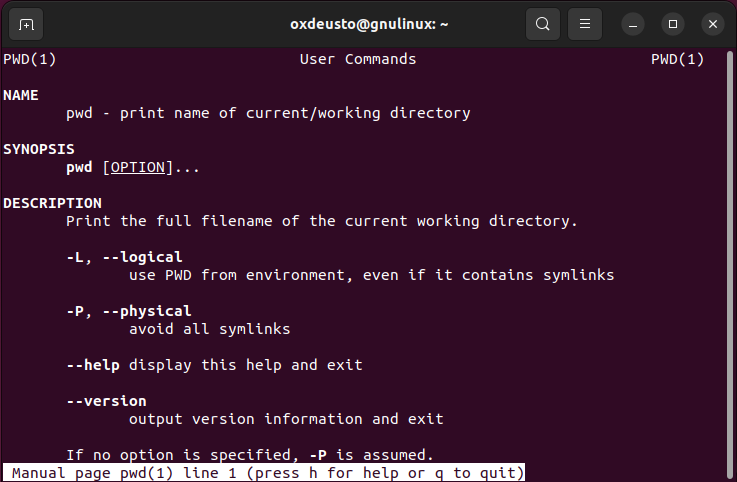
\includegraphics[width=0.80\linewidth]{resources/images/man.png}
    \caption{Manual de referencia del comando pwd.}
\end{figure}

man es muy útil porque nos permite consultar información de cada comando sin salir de la terminal, sin la necesidad tampoco de tener conexión a internet. Al abrir un manual, puede salir de él presionando la tecla q de (quit)

Es importante destacar que algunos pocos comandos no tienen una entrada en man, pero esto no es un problema, ya que ofrecen una opción de ayuda. Ésta normalmente es -h o --help.

Si bien man es una forma rápida de saber el uso general de un comando y la funcionalidad detallada de sus argumentos y opciones, las entradas del manual no suelen incluir ejemplos. Es por eso que, si deseas explicaciones más prácticas consultes internet. Foros de informática como StackOverflow (https://stackoverflow.com/) tienen respuestas a cualquier duda que se te pueda ocurrir. El foro de AskUbuntu (https://askubuntu.com/) tiene preguntas más relacionadas con Ubuntu, pero también es un buen lugar donde resolver dudas.

\section{Manipulando nuestro entorno de fichero}
Para sorpresa de nadie, una de las funcionalidades más importantes de un sistema operativo es poder crear, modificar y eliminar ficheros. El shell de bash, naturalmente, nos ofrece comandos para poder realizar estas tareas básicas. Vamos a mirarlas una a una:

\begin{command-info}
{mkdir}
{Crear directorios.}
{mkdir <dirección del directorio>}
{-p}
{man mkdir o mkdir --help}
\end{command-info}

mkdir (o MaKe DIRectory) nos permite crear directorios. Veamos un ejemplo. Si quiero crear un directorio llamado "documentos" en el directorio en el que me encuentro, podríamos usar mkdir con direccionamiento relativo:

\begin{tcolorbox-code}
\begin{lstlisting}
$ mkdir documentos
\end{lstlisting}
\end{tcolorbox-code}

Esto crea un directorio llamado "documentos" dentro del directorio en el que me encuentro. Recuerda que se puede conseguir el mismo resultado con direccionamiento absoluto. Si quiero crear el directorio en mi carpeta de usuario, puedo hacer...

\begin{tcolorbox-code}
\begin{lstlisting}
$ mkdir /home/oxdecode/documentos
\end{lstlisting}
\end{tcolorbox-code}

o...

\begin{tcolorbox-code}
\begin{lstlisting}
$ mkdir ~/documentos
\end{lstlisting}
\end{tcolorbox-code}

Si queremos crear más de un directorio a la vez, cada uno dentro de otro, tenemos que usar la opción -p. Observa:

\begin{tcolorbox-code}
\begin{lstlisting}
$ mkdir -p documentos/2024/mayo
\end{lstlisting}
\end{tcolorbox-code}

Este comando sería equivalente a hacer la siguiente sucesión de comandos:

\begin{tcolorbox-code}
\begin{lstlisting}
$ mkdir documentos
$ mkdir documentos/2024
$ mkdir documentos/2024/mayo
\end{lstlisting}
\end{tcolorbox-code}

Hemos aprendido a crear directorios, vamos a aprender ahora cómo crear ficheros:

\begin{command-info}
{touch}
{Crear ficheros (archivos).}
{touch <dirección del fichero>}
{Ninguna}
{man touch o touch --help}
\end{command-info}

El comando touch te permite crear ficheros en una dirección específica. El uso es el siguiente:

\begin{tcolorbox-code}
\begin{lstlisting}
$ touch documentos/2024/mayo/factura.txt
\end{lstlisting}
\end{tcolorbox-code}

Este fichero crea en ~/documentos/2024/mayo un fichero llamado "factura" de extensión .txt.

Hemos aprendido a crear directorios y ficheros. Más tarde aprenderemos a manejar los permisos de los ficheros, pero por ahora, veamos cómo eliminar ficheros o directorios.

\begin{center}
  \rule{15cm}{0.4pt}
\end{center}
\textbf{rm}\\
Utilidad: Elimina directorios o ficheros.\\
Forma de uso general: rm <dirección del directorio o fichero>\\
Opciones comunes: -r, -d\\
Ayuda: man rm o rm --help
\begin{center}
  \rule{15cm}{0.4pt}
\end{center}

\begin{command-info}
{rm}
{Elimina directorios o ficheros.}
{rm <dirección del directorio o fichero>}
{-r, -d}
{man rm o rm --help}
\end{command-info}

rm (ReMove) es el comando que utilizamos para eliminar directorios o ficheros. Para eliminar ficheros, nos basta con hacer lo siguiente:

\begin{tcolorbox-code}
\begin{lstlisting}
$ rm ~/documentos/2024/mayo/factura.txt
\end{lstlisting}
\end{tcolorbox-code}

Esto eliminará el fichero "factura.txt". Una vez más, recuerda que también se puede utilizar direccionamiento relativo para todas estas tareas. Para eliminar directorios, no nos basta con seguir la misma estructura:

\begin{tcolorbox-code}
\begin{lstlisting}
$ rm ~/documentos/2024/mayo/
rm: cannot remove ‘documentos/2024/mayo’: is a directory
\end{lstlisting}
\end{tcolorbox-code}

rm requiere la opción -r o -d para eliminar directorios. Si queremos eliminar un directorio de forma recursiva, tenga ficheros dentro o no, utilizamos -r (recursive).

\begin{tcolorbox-code}
\begin{lstlisting}
$ rm -r ~/documentos
\end{lstlisting}
\end{tcolorbox-code}

Esto va a eliminar "documentos" y todo lo que había en su interior.

Existe también la opción -d, que elimina sólo directorios vacíos. Es una opción más segura de utilizar el comando rm.

\textbf{\textbf{Nota:}} Existe el comando rmdir, que elimina directorios siempre que estén vacíos, como el comando rm -d.
Ya sabemos crear y eliminar directorios y ficheros. Antes de ver cómo copiarlos o moverlos, vamos a aprender a usar un comando muy útil, que si bien no modifica nuestro entorno de trabajo, es una herramienta muy importante.

\begin{command-info}
{ls}
{Enlista el contenido de un directorio}
{ls <dirección>}
{-R, -a, -l...}
{man ls o ls --help}
\end{command-info}

ls (LiSt) es un comando que nos permite ver el contenido de un directorio, tanto sus ficheros como otros directorios dentro. Para mostrarlo, vamos a movernos a root y listar el contenido:

\begin{tcolorbox-code}
\begin{lstlisting}
$ cd /
$ ls
\end{lstlisting}
\end{tcolorbox-code}

Obtendremos esto:
\begin{figure}[H]
    \centering
    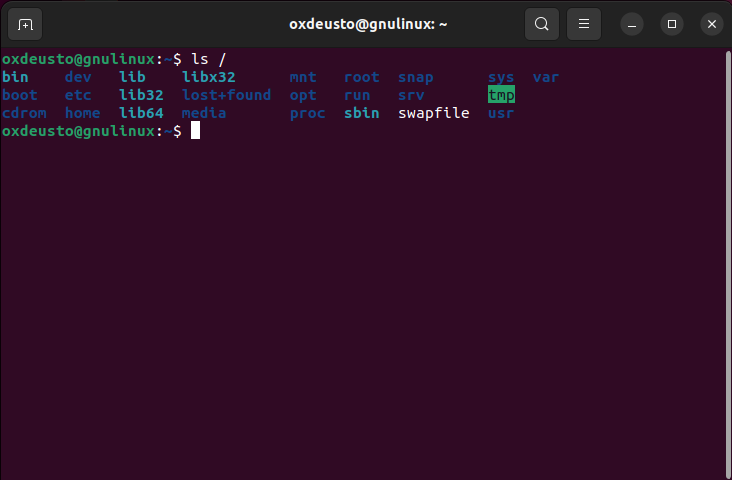
\includegraphics[width=0.8\linewidth]{resources/images/ls_1.png}
    \caption{Comando ls.}
\end{figure}

La mayoría de los elementos (los que están en azul oscuro) son directorios, de los cuales se pueden ver algunos que ya conocemos por el Tema 1, como /bin, /etc /home... Esto es root (/), y todos los datos del sistema operativo los puedes encontrar aquí, en alguno de estos directorios.

ls es un comando con bastantes opciones, y es recomendable consultar su manual ya que hay opciones de mucha utilidad. Vamos a consultar algunas de las más importantes.

Con la opción -R podemos listar recursivamente cada directorio dentro del directorio que estamos enlistando. Es decir, que además de listar el contenido del directorio deseado, lista también el contenido de los directorios dentro de éste. Como listar recursivamente / implicaría tener que listar literalmente nuestro sistema operativo entero, sería conveniente probarlo en un directorio menos denso, como podría ser nuestra carpeta "documentos":

\begin{tcolorbox-code}
\begin{lstlisting}
$ ls -R ~/documentos
\end{lstlisting}
\end{tcolorbox-code}
\begin{figure}[H]
    \centering
    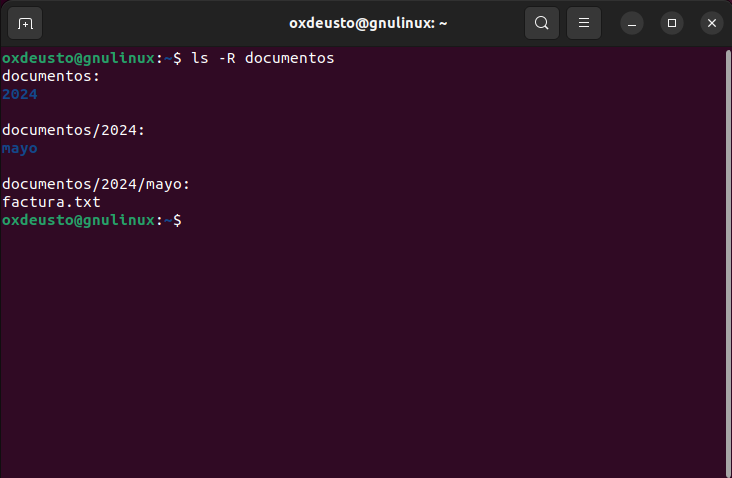
\includegraphics[width=0.80\linewidth]{resources/images/ls_2.png}
    \caption{ls recursivo.}
\end{figure}

Al usar la opción -R podemos ver el contenido de cada subdirectorio en documentos.

Con la opción -a podemos listar los ficheros ocultos del directorio. Un fichero oculto es un fichero que tiene como primer carácter en el nombre un punto. Para realizar la prueba, vamos a crear un fichero oculto en ~:

\begin{tcolorbox-code}
\begin{lstlisting}
$ touch ~/.secreto.txt
$ ls ~
\end{lstlisting}
\end{tcolorbox-code}

Al listar el directorio, verás como el fichero recién creado no se muestra.

\begin{figure}[H]
    \centering
    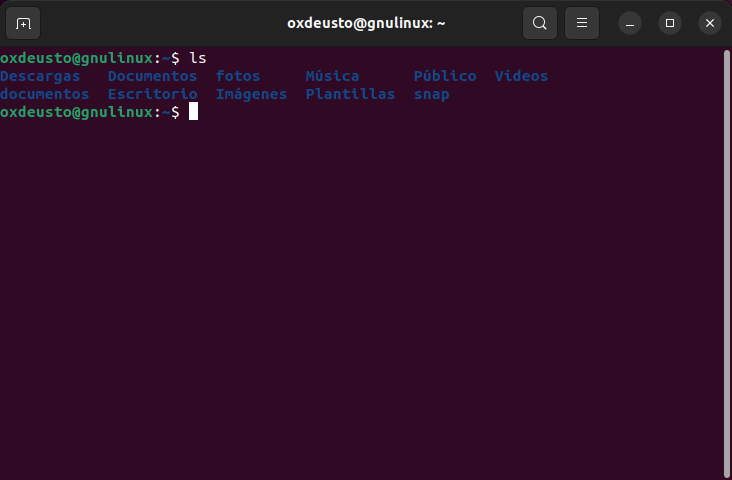
\includegraphics[width=0.80\linewidth]{resources/images/ls_3.png}
    \caption{ls normal, no se muestran ficheros ocultos.}
\end{figure}

Esto se debe a que ls no imprime ficheros ocultos a no ser que utilicemos la opción -a:
\begin{tcolorbox-code}
\begin{lstlisting}
$ ls -a ~
\end{lstlisting}
\end{tcolorbox-code}

\begin{figure}[H]
    \centering
    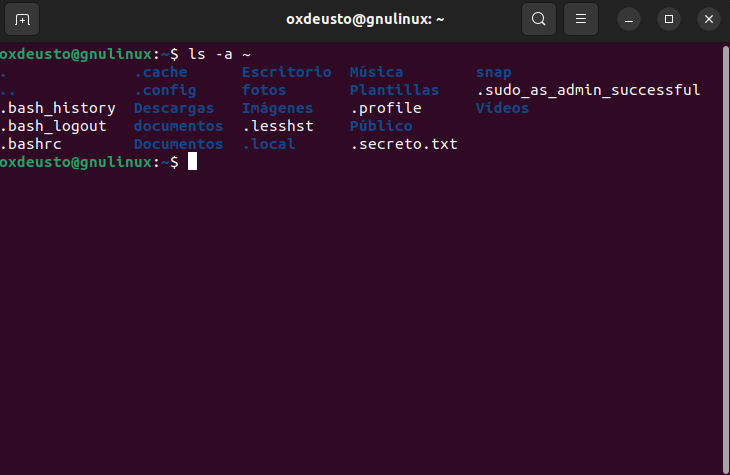
\includegraphics[width=0.80\linewidth]{resources/images/ls_4.png}
    \caption{ls -a, nos muestra también los ficheros ocultos.}
\end{figure}

Fíjate cómo además de .secreto.txt, \~ contiene otros ficheros ocultos que no hemos creado nosotros. Estos ficheros tienen diferentes utilidades, por ejemplo .bash\_history es un log de los comandos que hemos utilizado en la terminal. .bashrc es un script que se ejecuta cuando iniciamos sesión. .bash\_logout se ejecuta cuando se cierra una shell. Para nuestro contexto, estos ficheros no nos interesan, pero pueden ser muy útiles en algunas situaciones.

Cabe destacar que es posible utilizar más de una opción en un comando, obteniendo así la funcionalidad de ambas opciones:

\begin{tcolorbox-code}
\begin{lstlisting}
$ ls -aR # ls -a -R tambíen sirve
\end{lstlisting}
\end{tcolorbox-code}

Además de crear y eliminar directorios y ficheros, nos puede ser de utilidad copiarlos y moverlos, además de renombrarlos:

\begin{command-info}
{cp}
{Copia un fichero o directorio a una dirección.}
{cp <dir. origen> <dir. destino>}
{-r}
{man cp o cp --help}
\end{command-info}

cp (CoPy) es un comando que nos permite copiar un fichero o un directorio. Como esta operación implica dos direcciones, el formato que utiliza es uno diferente al que hemos visto hasta ahora. Vamos a copiar el fichero factura.txt a nuestra carpeta de usuario, estando en esa misma carpeta:

\begin{tcolorbox-code}
\begin{lstlisting}
$ cp documentos/2024/mayo/factura.txt .
\end{lstlisting}
\end{tcolorbox-code}

Fíjate cómo en la dirección de destino colocamos nada más que un punto. Este punto representa un "aquí". Cuando colocamos un punto en la dirección de destino estamos indicando que queremos copiar el fichero en el directorio en el que nos encontramos, en este caso en ~.

Para copiar directorios hay que usar una opción, -r.

\begin{tcolorbox-code}
\begin{lstlisting}
$ cp -r documentos .
\end{lstlisting}
\end{tcolorbox-code}

\begin{command-info}
{mv}
{Mueve un directorio o fichero a otra dirección.}
{mv <dir. origen> <dir. destino>}
{Ninguna}
{man mv o mv --help}
\end{command-info}

mv (MoVe) sigue la misma estructura que cp, pero en vez de copiar el fichero o el directorio, cambia su dirección. Esto tiene una funcionalidad extra muy importante. Cambiar nombres. Al fin y al cabo, si cambias la dirección de un fichero o directorio, tienes la posibilidad de cambiar su nombre también.

\begin{tcolorbox-code}
\begin{lstlisting}
$ mv documentos/2024/mayo/factura.txt ./factura\_mayo\_2024.txt
\end{lstlisting}
\end{tcolorbox-code}

En este caso estoy moviendo factura.txt al directorio en el que estoy (~), dándole el nombre de "factura\_mayo\_2024.txt". No hace falta cambiar el directorio del fichero para cambiar su nombre:

\begin{tcolorbox-code}
\begin{lstlisting}
$ cd documentos/2024/mayo
$ mv factura.txt factura_mayo_2024.txt
\end{lstlisting}
\end{tcolorbox-code}

Gracias a todo estos comandos (mkdir, touch, rm, ls, cp y mv) ya sabemos cómo modificar nuestro entorno de archivos. En el próximo apartado nos vamos a centrar en la modificación de ficheros. Está bien ser capaz de crear y eliminar ficheros, pero si no sabemos cómo modificar su contenido, no nos pueden ser de mucha utilidad.

\section{Editar ficheros}
Editar ficheros es una funcionalidad clave en cualquier sistema operativo. Gracias a ésta podemos sacarle provecho a los ficheros, para almacenar información o incluso programar en ellos. Para esto utilizamos los editores de texto (IDE). Uno muy conocido y utilizado por muchos programadores y programadoras es Visual Studio Code, que te ofrece incontables herramientas para optimizar tu programación. VS Code, al igual que muchos otros IDEs como Eclipse, NetBeans o IntelliJ, contiene interfaces gráficas que facilitan su uso para el usuario promedio, pero también existen editores de texto para terminales.



Uno de los más utilizados gracias a lo extremadamente personalizable que es, es vim (o neovim). Este IDE ha ganado fama entre los programadores/as que pasan la mayor parte de su tiempo en la terminal. Puede convertirse en un entorno de programación muy rápido, superando en eficiencia incluso a los IDEs con interfaces gráficas. Sin embargo, aprender a utilizarlo no es un proceso fácil. Por ello, vamos a fijarnos en un editor de texto que suele venir por defecto en muchas distribuciones, que es perteneciente al proyecto GNU: nano.

\begin{command-info}
{nano}
{Abre el editor de texto "nano".}
{nano <fichero a editar (opcional)>}
{Ninguna}
{man nano o nano --help}
\end{command-info}

nano es un editor de texto básico, que en la práctica no es del todo recomendable usarlo, y menos para programar. Pero para este curso nos sirve como ejemplo de editor de texto. Para abrirlo basta con escribir...

\begin{tcolorbox-code}
\begin{lstlisting}
$ nano
\end{lstlisting}
\end{tcolorbox-code}

...pero se suele especificar una dirección a un fichero, exista o no, para guardarlo directamente al terminar sin tener que especificar su nombre dentro del editor.

Independientemente de si especifiquemos una dirección o no, se nos abrirá una interfaz como esta:

\begin{figure}[H]
    \centering
    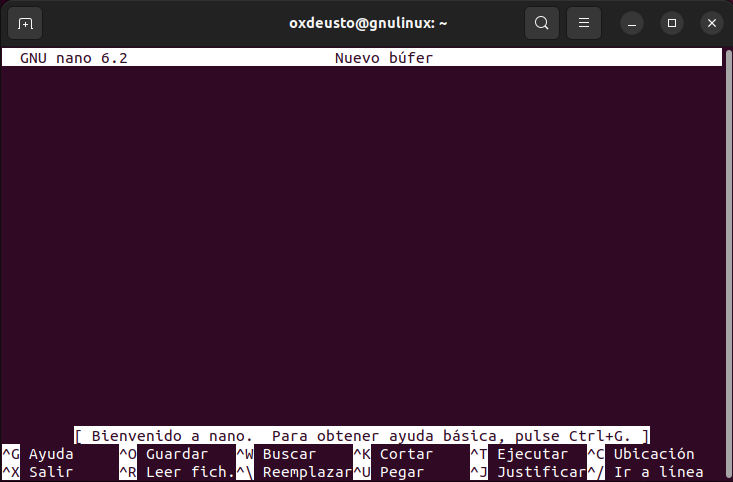
\includegraphics[width=0.80\linewidth]{resources/images/nano.png}
    \caption{Vista de nano.}
\end{figure}

En esta interfaz ya podemos escribir en el fichero como si fuera un editor de texto normal y corriente. En la parte inferior de la interfaz vemos unas cuantas opciones. Cada instrucción tiene el carácter "\^" acompañado de una letra. Ese carácter representa la tecla ctrl, es decir, que si queremos guardar el fichero tenemos que pulsar la combinación de teclas ctrl + o.

Como se puede observar, este editor de texto es muy sencillo de usar, así que tampoco hace falta que le dediquemos mucho tiempo a ver sus funcionalidades.

Para futuros ejemplos, vamos a escribir algo en este fichero y lo vamos a guardar en la dirección del fichero de facturas.txt. De esta manera, vamos a sobreescribirlo con el texto que hemos escrito con nano:

\begin{figure}[H]
    \centering
    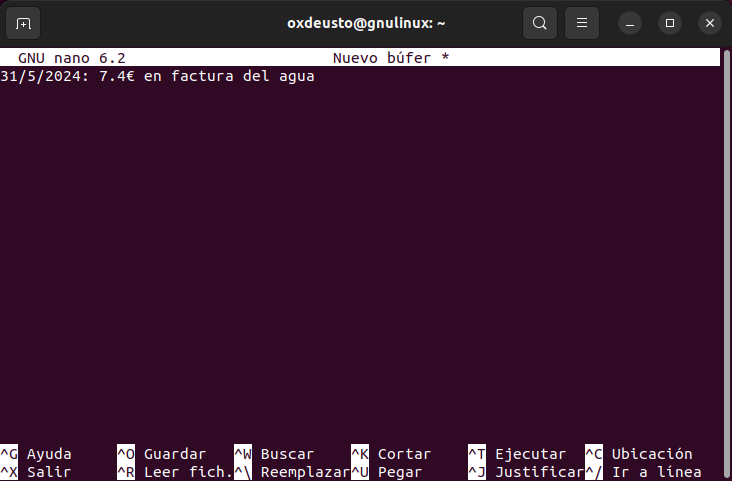
\includegraphics[width=0.80\linewidth]{resources/images/nano_2.png}
    \caption{Texto escrito en nano.}
\end{figure}

Le damos a ctrl + o y escribimos la dirección.

\begin{figure}[H]
    \centering
    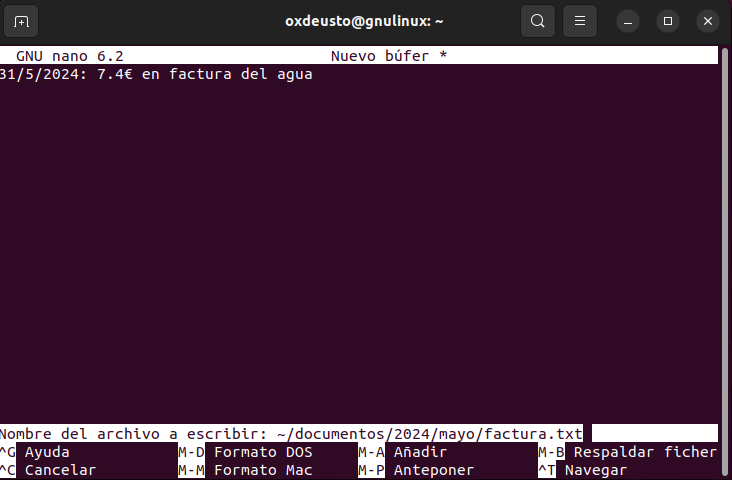
\includegraphics[width=0.75\linewidth]{resources/images/nano_3.png}
    \caption{Entrada de dirección del fichero.}
\end{figure}

\textbf{Nota:} En apartados anteriores hubo un ejemplo en el que movimos este fichero a ~, así que si estás ejecutando los comandos de estos apuntes en tu máquina, tendrás dos facturas, una en ~ y otra en ~/documentos/2024/mayo/, y en este ejemplo no estarás sobreescribiendo el fichero, lo estarías creando de nuevo en el directorio "mayo". Sin embargo, el resultado no cambia.

Ahora que hemos aprendido a escribir archivos, vamos a aprender a leerlos sin usar un editor de texto:

\begin{command-info}
{cat}
{Imprime los ficheros que recibe como parámetro.}
{cat <dir. fichero> <dir. fichero2>}
{Ninguna}
{man cat o cat --help}
\end{command-info}

cat (conCATenate) concatena (une) el contenido de los ficheros que recibe como parámetros y los imprime. Si bien puedes consultar el contenido de un fichero mediante un editor de texto, cat es el comando que se usa para imprimir un fichero en consola, porque nos puede permitir usar el contenido de un fichero como datos de entrada para algún comando mediante el uso de los pipes (más sobre esto más tarde). El uso es muy sencillo, vamos a imprimir el fichero que acabamos de crear:

\begin{tcolorbox-code}
\begin{lstlisting}
$ cat ~/documentos/2024/mayo/factura.txt
31/5/2024: 7.4 € en factura del agua
\end{lstlisting}
\end{tcolorbox-code}

Si creo otro fichero llamado factura2.txt con el texto "31/5/2024: 78.34 € en factura de la luz" y lo añado como argumento junto con factura.txt, el resultado es de esperar:

\begin{tcolorbox-code}
\begin{lstlisting}
$ cat factura.txt factura2.txt # Estando en el directorio mayo/
31/5/2024: 7.4 € en factura del agua
31/5/2024: 78.34 € en factura de la luz
\end{lstlisting}
\end{tcolorbox-code}

\section{Usuarios}
GNU/Linux, al igual que los demás sistemas operativos principales del mercado, ofrece un sistema de usuarios. Sin embargo, Linux da un paso más en cuanto al control sobre éstos, ofreciéndonos más utilidades sobre los permisos de cada usuario.

En Linux hay tres tipos de usuarios:

\begin{itemize}
    \item \textbf{Usuario root}: Es el usuario con permisos absolutos sobre el sistema. Además de esto, se distingue de los demás usuarios por tener el UID (User ID) 0. En nuestros usuarios personales, cuando queremos realizar una tarea que requiere permisos especiales (de nivel root), utilizamos el comando sudo <comando> para heredar permisos de root para ese comando, una vez proporcionada la contraseña de root.

    \item \textbf{Usuarios personales}: Son los usuarios que creamos nosotros. En la mayoría de los casos tienen sus directorios propios en /home y sus UIDs parten del número 1000. En función de nuestras configuraciones, cada usuario tiene permisos diferentes ante diferentes ficheros.

    \item \textbf{Usuarios del sistema}: Son usuarios que crea el propio sistema operativo o programas que tengamos instalados, y pueden tener muchos usos diferentes dependiendo de su origen. Sus UIDs son menores de 1000 y normalmente tienen permisos de sudo, pero este no es siempre el caso. Para este curso este tipo de usuario no nos interesa, pero sé consciente de que estos usuarios existen y tienen un papel importante en el funcionamiento de muchos programas.
\end{itemize}

Ahora vamos a ver cómo crear un usuario personal en Linux:

\begin{command-info}
{useradd}
{Permite crear usuarios.}
{sudo useradd <nombre de usuario>}
{-m}
{man useradd o useradd --help}
\end{command-info}

useradd fundamentalmente nos permite crear usuarios, pero vamos a necesitar otros comandos si queremos configurar un usuario por completo. En cualquier caso, creamos un usuario de la siguiente manera:

\begin{tcolorbox-code}
\begin{lstlisting}
$ sudo useradd -m franz
\end{lstlisting}
\end{tcolorbox-code}

Con este comando creamos un usuario llamado "franz". Nótese cómo usamos sudo para este comando. Crear usuarios requiere permisos de root, por lo cual necesitaremos introducir de nuevo nuestra contraseña, y que formemos parte del grupo de sudoers (lo veremos más adelante). 

También usamos la opción -m. Esta opción, además de crear el usuario, crea un directorio de usuario para él, en /home. Ahora vamos a darle una contraseña a este usuario:

\begin{command-info}
{passwd}
{Crea o modifica contraseñas de usuarios.}
{sudo passwd}
{-d}
{man passwd o passwd}
\end{command-info}

\begin{tcolorbox-code}
\begin{lstlisting}
$ sudo passwd franz
\end{lstlisting}
\end{tcolorbox-code}

Este comando te pedirá una contraseña y que la repitas, para asignarla a Franz. Se puede eliminar la contraseña del usuario utilizando la opción -d (delete).

Con estos dos comandos básicos podemos crear un usuario y establecer su contraseña. Ahora vamos a aprender a configurar otras características de usuarios:

\begin{command-info}
{usermod}
{Permite modificar características de usuarios.}
{sudo usermod [opción(es)] <usuario>}
{-aG, -l...}
{man usermod o usermod --help}
\end{command-info}

usermod tiene varios usos. Uno de los más importantes es poder cambiar el grupo al que pertenece el usuario. Los grupos los veremos en detalle en el próximo apartado, pero por ahora, hay un grupo en concreto que permite a sus usuarios poder usar el comando sudo. Para darle a Franz permisos de sudo, podemos usar el siguiente comando:

\begin{tcolorbox-code}
\begin{lstlisting}
$ sudo usermod -aG sudo franz
\end{lstlisting}
\end{tcolorbox-code}

La opción -G nos indica que queremos meter a Franz en los grupos que le indicamos (separado por comas). En este caso, queremos añadirle al grupo de sudo (sudoers). Los usuarios dentro de este grupo tienen acceso al comando sudo. Añadimos la opción -a (append) para añadirle a Franz al grupo sudo sin que se salga de los demás grupos en los que está. De no incluir -a, Franz se añadiría a sudo pero abandonaría sus otros grupos.

usermod tiene muchos otros usos, estos son algunos más:

\begin{tcolorbox-code}
\begin{lstlisting}
$ sudo usermod -u 1024 franz # Cambia el UID de franz a 1024
$ sudo usermod -l nuevo_nombre franz # Cambia el nombre de franz
$ sudo usermod -L franz # Deshabilita la cuenta de franz
$ sudo usermod -U franz # Rehabilita la cuenta de franz
\end{lstlisting}
\end{tcolorbox-code}

Existen bastantes usos más para este comando, así que es recomendable consultar la página del manual de usermod para más información.

Ahora que hemos aprendido a cambiar de usuarios, vamos a ver cómo cambiar de usuario en la terminal:

\begin{command-info}
{su}
{Permite cambiar de usuario.}
{su <usuario al que quieres cambiar>}
{Ninguna}
{man usermod o usermod --help}
\end{command-info}

su (Switch User) nos abre una shell dentro de nuestra terminal que nos permite ejecutar comandos bajo otro usuario, una vez escribes su contraseña.

\begin{tcolorbox-code}
\begin{lstlisting}
$ su franz
$ # Shell nueva bajo el usuario franz
\end{lstlisting}
\end{tcolorbox-code}

Una forma de comprobar que hemos cambiado de usuario correctamente es mediante el comando whoami:

\begin{command-info}
{whoami}
{Imprime el nombre de usuario de tu shell actual}
{whoami}
{Ninguna}
{man whoami o whoami --help}
\end{command-info}

\begin{tcolorbox-code}
\begin{lstlisting}
$ whoami
franz
$
\end{lstlisting}
\end{tcolorbox-code}

Hemos ejecutado whoami bajo el usuario franz, por ello nos devuelve "franz" y no "oxdecode". Ahora sabemos que hemos cambiado de usuario correctamente.

Si queremos volver a nuestro usuario original, basta con escribir "exit", o pulsando la combinación de teclas ctrl + D. Veremos cómo nuestro shell prompt vuelve a aparecer.

Para terminar vamos a ver cómo eliminar un usuario:

\begin{command-info}
{userdel}
{Elimina un usuario.}
{sudo userdel <usuario>}
{-r, -f}
{man userdel o userdel --help}
\end{command-info}

Si queremos eliminar un usuario, normalmente se hace de esta manera:

\begin{tcolorbox-code}
\begin{lstlisting}
$ sudo userdel -r franz
\end{lstlisting}
\end{tcolorbox-code}

La opción -r, además de eliminar el usuario, elimina también su carpeta de usuario. De no incluir esta opción, los ficheros en el directorio se quedarían sin propietario.

\section{Grupos}

A diferencia de Windows, los usuarios de Linux pueden formar parte de unos conjuntos llamados grupos. Los grupos nos facilitan la gestión de usuarios.

Un ejemplo para el uso de grupos podría ser en una empresa. Imagínate que en un sistema de una empresa trabajan dos tipos de trabajadores: administradores/as y técnicos/as. Tendría sentido que los administradores/as tengan acceso a ficheros más privados de la empresa, o que puedan ejecutar programas que los técnicos/as no. Para esto podemos crear grupos, ya que con ellos podemos establecer un sistema de permisos generalizado para cada grupo.

Uno de los grupos que viene por defecto en nuestro sistema es el grupo sudo (a veces llamado "wheel"), que contiene en él todos los usuarios con permisos para ejecutar comandos con sudo. Por eso, cuando queremos hacer que un usuario tenga acceso al comando sudo, basta con añadirle a este grupo.

Además de esto, los grupos tienen otro concepto importante que tiene que ver con los usuarios, los grupos primarios. Cada usuario tiene un grupo primario que, si no se especifica lo contrario, tiene como nombre el mismo nombre que el usuario. Cuando un usuario crea un fichero, el propietario de ese fichero será el grupo principal del usuario (hablaremos de esto más adelante, en el apartado de permisos).

Antes de continuar, el grupo primario de un usuario se cambia así:

\begin{tcolorbox-code}
\begin{lstlisting}
$ sudo usermod -g grupo_primario_nuevo oxdecode
\end{lstlisting}
\end{tcolorbox-code}

Ahora vamos a aprender a cómo configurar grupos. Vamos a empezar por cómo crearlos:

\begin{command-info}
{groupadd}
{Permite crear grupos.}
{sudo groupadd <nombre del grupo>}
{Ninguna}
{man groupaddo groupadd --help}
\end{command-info}

El uso de groupadd es muy sencillo, nos puede recordar incluso a useradd.

\begin{tcolorbox-code}
\begin{lstlisting}
$ sudo groupadd administradores
\end{lstlisting}
\end{tcolorbox-code}

Con este comando ya hemos creado un grupo. Si queremos añadir un usuario a este grupo, podemos hacerlo con un comando que ya hemos visto antes, usermod:

\begin{tcolorbox-code}
\begin{lstlisting}
$ sudo usermod -aG administradores oxdecode
\end{lstlisting}
\end{tcolorbox-code}

Al igual que para los usuarios, los grupos tienen un comando específico para modificar sus características: groupmod:

\begin{command-info}
{groupmod}
{Permite modificar características de grupos.}
{sudo groupmod [opción(es)] <grupo>}
{-n, -g}
{man groupmod o groupmod --help}
\end{command-info}

Con groupmod, entre otras cosas, podemos cambiar el nombre del grupo o su GID (Group ID)

\begin{tcolorbox-code}
\begin{lstlisting}
$ sudo groupmod -n staff administradores
$ sudo groupmod -g 1049 staff
\end{lstlisting}
\end{tcolorbox-code}

Aquí renombramos administradores a "staff" y le asignamos la GID 1049. 

Ahora vamos a ver lo que hacen un comando de utilidad para los grupos: groups e id:

\begin{command-info}
{groups}
{Muestra los grupos a los que pertenece un usuario.}
{groups <usuario>}
{Ninguna}
{man groups o groups --help}
\end{command-info}

groups es un comando simple que imprime los grupos de un usuario:

\begin{tcolorbox-code}
\begin{lstlisting}
$ groups oxdecode
oxdecode sudo administradores
\end{lstlisting}
\end{tcolorbox-code}

Al ejecutar el comando podemos ver que el usuario oxdecode forma parte de tres grupos: oxdecode (su grupo primario), sudo (porque oxdecode es sudoer) y administradores (porque lo hemos añadido antes).

\begin{command-info}
{id}
{Muestra los grupos a los que pertenece un usuario.}
{id <usuario>}
{Ninguna}
{man id o id --help}
\end{command-info}

id tiene una funcionalidad similar, pero también nos imprime nuestro UID (User ID) y los GIDs (Group IDs) de nuestros grupos:

\begin{tcolorbox-code}
\begin{lstlisting}
$ id oxdecode
uid=1000(oxdecode) gid=1009(oxdecode) groups=1009(oxdecode),27(sudo),1011(administradores)
\end{lstlisting}
\end{tcolorbox-code}

Fíjate cómo imprime dos veces la GID del grupo oxdecode. La primera indica que es el grupo primario, mientras que despues de "groups=" está mencionando todos los grupos, incluido el primario.

Veamos cómo podemos eliminar grupos ahora:

\begin{command-info}
{groupdel}
{Elimina un grupo.}
{sudo groupdel <grupo>}
{Ninguna}
{man groupdel o groupdel --help}
\end{command-info}

groupdel elimina un grupo, y su forma de uso es muy sencilla:

\begin{tcolorbox-code}
\begin{lstlisting}
$ sudo groupdel administradores
\end{lstlisting}
\end{tcolorbox-code}

Sin embargo, hay que tener algo en cuenta: antes de eliminar un grupo, tienes que asegurarte de que no hay usuarios en éste. Para ello tienes que modificar los grupos de cada usuario que pertenezca al grupo que quieres eliminar. Esto se hace para evitar problemas con los permisos de grupos en ficheros.

\section{Ficheros para usuarios y grupos}
Como hemos visto, para crear y modificar usuarios o grupos, es necesario tener permisos de root. ¿A qué se debe esto? La razón es la siguiente: los comandos que hemos aprendido sobre usuarios y grupos (useradd, usermod, groupadd, groupmod...) trabajan en unos ficheros en concreto dentro del directorio /etc. Estos son los ficheros importantes con los que se trabaja:

/etc/passwd: en passwd se encuentra la información básica de cada usuario. Vamos a ver el contenido del fichero:

\begin{tcolorbox-code}
\begin{lstlisting}
$ cat /etc/passwd
(...)
oxdecode:x:1000:1009:0xDECODE,,,:/home/oxdecode:/bin/bash
franz:x:1006:1010::/home/franz:/bin/sh
\end{lstlisting}
\end{tcolorbox-code}

Te saldrán muchas líneas, la mayoría de ellas son usuarios de sistema, pero en las últimas podremos ver nuestros usuarios.
Cada línea representa un usuario, y todas las líneas siguen el mismo formato:

\begin{tcolorbox-code}
\begin{lstlisting}
username:x:UID:GID_primario:comentarios:dir_usuario:shell
\end{lstlisting}
\end{tcolorbox-code}

Fijándonos en la línea del usuario oxdecode, vemos que su nombre de usuario es "oxdecode". Justo después, vemos una "x". Esto indica que la contraseña del usuario está almacenada de forma segura en otro fichero con el que los comandos de usuarios y grupos trabajan: /etc/shadow. Después nos sale el UID y el GID del grupo primario del usuario. Luego van los comentarios. Como la cuenta oxdecode la creé usando un comando diferente a useradd que nos proporciona Ubuntu/Debian (adduser), salen unos comentarios. Esta parte la puedes ignorar si has creado tu usuario con useradd y no has proporcionado comentarios al usuario. Franz, que la creé con useradd, no tiene comentarios. Después de los comentarios se encuentra la dirección al directorio del usuario, y después el shell que usa, en este caso bash. El shell por defecto no es bash, es sh, una versión más primitiva en la que bash está basada.

/etc/group: En este fichero se encuentran los grupos del sistema:

\begin{tcolorbox-code}
\begin{lstlisting}
$ cat /etc/passwd
(...)
oxdecode:x:1009:
franz:x:1010:
administradores:x:1011:oxdecode,franz
\end{lstlisting}
\end{tcolorbox-code}

Como veremos, existen muchos grupos de sistema, pero en las últimas líneas estarán los grupos que hemos creado nosotros. Cada línea sigue este formato:

\begin{tcolorbox-code}
\begin{lstlisting}
nombre\_grupo:x:GID:miembro1,miembro2,...,miembroN
\end{lstlisting}
\end{tcolorbox-code}

Los dos primeros grupos que salen en el output de arriba (oxdecode y franz) son los grupos primarios de los usuarios con sus respectivos nombres ("oxdecode" y "franz"). Después vuelve a aparecer el indicador de que nuestra contraseña está cifrada en /etc/shadow y después la GID del grupo.

Para el caso de administradores, vemos también los miembros del grupo, en este caso oxdecode y franz también.

/etc/shadow: shadow es un fichero que no vamos a ver a fondo en este curso, pero las características fundamentales del fichero son que, a diferencia de passwd y groups, necesitamos permisos de sudo para leer este fichero, y que shadow se encarga de guardar la información sobre la contraseña de usuarios y grupos, junto con una versión cifrada de ésta.

\section{Conclusión y resumen de usuarios/grupos}
Esto es todo sobre usuarios y grupos. Los usuarios y grupos son una parte muy importante del sistema y lo que hemos visto ha sido sólo lo fundamental. Como es mucha información, aquí hay un breve resumen sobre lo que hemos dado.

\begin{itemize}
    \item Los usuarios de Linux son entidades que usamos para realizar tareas. Hay tres tipos de usuarios: el root, los usuarios de sistema y los usuarios personales.

    \item Para crear un usuario usamos el comando useradd, junto con usermod para configurarlo.

    \item Usamos el comando su para movernos entre usuarios, y el comando whoami para saber qué usuario estamos utilizando.

    \item Los grupos de usuarios son conjuntos de usuarios que nos ayudan a gestionar los permisos de los usuarios de forma más sencilla. Cada usuario tiene un grupo primario, y un conjunto de grupos secundarios.

    \item Creamos grupos usando el comando groupadd, y groupmod para modificar su configuración.

    \item Para hacer cambios en los grupos de un usuario utilizamos usermod, y podemos consultar los grupos a los que pertenecemos utilizando el comando groups.

    \item Tanto los usuarios como los grupos tienen unos ficheros donde guardan la información, estos ficheros (entre otros) son /etc/passwd para usuarios y /etc/group para los grupos.
\end{itemize}

\section{Permisos}
Linux nos ofrece un sistema de permisos para ficheros y directorios muy intuitivo y útil. Gracias a las utilidades que nos ofrece, nosotros, los usuarios, podemos gestionar quién puede hacer qué en nuestros ficheros.

En un sistema operativo, los tres permisos fundamentales son los de lectura, escritura y ejecución. Los permisos de lectura nos permiten poder saber cuál es el contenido de un fichero. Los de escritura nos permiten editarlo, y los de ejecución simplemente nos permiten ejecutar esos ficheros.

Estos tres permisos nos indican qué es lo que puede hacer un usuario. Vamos a ver cómo indicar quién es el que tiene esos permisos:

Por cada fichero, se asignan (o no) permisos de lectura, escritura y ejecución a tres grupos de usuarios: El propietario/a, el grupo de usuarios que comparten grupo con el propietario/a, y los demás usuarios. Esto significa que los dos factores que determinan los permisos que tienes sobre un fichero son los grupos a los que perteneces y si eres el propietario/a.

Una de las primeras preguntas que nos puede surgir una vez conocemos esta información es cómo consultar los permisos de un fichero. Para ello tenemos que usar una opción en concreto del comando ls.

\begin{tcolorbox-code}
\begin{lstlisting}
$ cd ~/documentos/2024/mayo/factura.txt
$ ls -l factura.txt
-rw-rw-r-- 1 oxdecode oxdecode 38 dic 17 18:54 (...)
\end{lstlisting}
\end{tcolorbox-code}

Esta opción, al darle la dirección de un fichero, nos imprime varios detalles sobre el fichero, entre ellos los permisos que tiene. Fijémonos en la primera cadena de caracteres:

\begin{tcolorbox-code}
\begin{lstlisting}
-rw-rw-r--
\end{lstlisting}
\end{tcolorbox-code}

Vemos un total de diez caracteres. Estos son los permisos de cada conjunto que hemos mencionado antes. El primero de todos (-) es un indicador de qué es el elemento que estamos listando. Si es un guión, significa que es un fichero, y si es una "d" un directorio. Existe también la "l", que indica que es un enlace simbólico, un elemento que no vamos a ver en este curso. Como es un guión, sabemos que factura.txt es un fichero. 

Los tres caracteres siguientes (rw-) indican cuales son los permisos del propietario del fichero. En este caso, el propietario tiene permisos de lectura (r, viene de "Read") y escritura (w, viene de "Write"). Estos son los permisos por defecto del propietario cuando creamos cualquier fichero. Si tuviéramos los permisos completos, es decir, también el de ejecución, la cadena se vería así: (rwx), donde la x viene de "eXecute". Es decir, que los permisos que no tenemos se representan con un guión, en vez de con la letra asociada al permiso.

En los siguientes tres caracteres vemos (rw-) otra vez. Estos son los permisos del grupo del propietario.

Los caracteres restantes (r--) son los permisos de los demás usuarios, los que no son o el propietario o forman parte de su grupo. Por defecto, estos usuarios solo tienen permisos de lectura.

El comando ls -l también nos imprime el usuario propietario y el grupo propietario:

\begin{tcolorbox-code}
\begin{lstlisting}
oxdecode oxdecode
\end{lstlisting}
\end{tcolorbox-code}

Como podemos ver, "oxdecode" es el propietario de este fichero, y el grupo propietario también es "oxdecode", porque cuando creamos un usuario, por defecto, se crea un grupo con su mismo nombre y éste se configura como grupo primario del usuario.

Así somos capaces de consultar los permisos de un fichero, ahora vamos a ver cómo cambiarlos:

\begin{command-info}
{chmod}
{Modifica los permisos de ficheros y directorios.}
{(sudo) chmod [permisos] <fichero>}
{Opciones de modificación de permisos}
{man chmod o chmod --help}
\end{command-info}

chmod (CHange MODe) es un comando un poco diferente a los que hemos visto hasta ahora, pero en esencia, sigue la misma estructura: el comando, las opciones y una dirección. Sin embargo, hay unas cosas importantes que mencionar.

Dependiendo del fichero que estés modificando, es posible que necesites ejecutar el comando mediante sudo. Si eres el propietario del fichero, no necesitarás usarlo, porque tienes total libertad de modificar el fichero a tu antojo, incluidos sus permisos. Sin embargo, un usuario que no es el propietario de un fichero, no debería de ser capaz de poder modificar los permisos de éste, ya que no le pertenece. Es por eso que tendría que usar los permisos de root, el usuario con permisos absolutos en el sistema.

Otro factor a tener en cuenta es que si bien este comando puede usar las opciones convencionales que hemos visto hasta ahora, las opciones que usamos para cambiar los permisos en sí siguen unas notaciones diferentes a las que hemos visto hasta ahora. Vamos a ver las dos posibles:

Notación simbólica: La notación simbólica es una forma visualmente intuitiva de modificar los permisos de un fichero.

\begin{tcolorbox-code}
\begin{lstlisting}
$ chmod u+x factura.txt
$ chmod g-w factura.txt
$ chmod o=rw factura.txt
\end{lstlisting}
\end{tcolorbox-code}

Vamos a ver comando por comando su funcionalidad. En el primero, estamos añadiendo al propietario el permiso de ejecución del fichero. Si el primer carácter de la notación es una "u", estamos cambiando los permisos del propietario. El "+" significa que estamos añadiendo algo (append), en este caso el permiso de ejecución, representado con una "x". Es decir, que tras este comando, el propietario (u) tendrá los permisos que tenía antes más el permiso de ejecución.

En el segundo comando estamos haciendo lo contrario. El primer carácter "g", indica que estamos realizando un cambio en los permisos del grupo del propietario. En este caso, estamos eliminando su permiso de escritura en el fichero (por eso usamos un "-"). Al ejecutarse este comando, los miembros del grupo del propietario tendrán los permisos que tenían antes menos el de escritura.

En el tercer comando, con la "o" estamos modificando los permisos de los demás usuarios (others) que no son ni el propietario ni forman parte de su grupo. En este caso no estamos ni añadiendo ni eliminando permisos, los estamos configurando desde cero. Con el "=", se sobreescriben los permisos del objetivo. En este caso, estamos dándole a los others permisos de lectura y escritura, sobreescribiendo los que tenía antes.

Se pueden cambiar los ficheros de varias entidades a la vez mediante el uso de comas. Por ejemplo, los tres comandos del ejemplo anterior se pueden resumir a uno de la siguiente manera:

\begin{tcolorbox-code}
\begin{lstlisting}
$ chmod u+x,g-w,o=rw factura.txt
\end{lstlisting}
\end{tcolorbox-code}

Sin embargo, esta forma puede ser algo enrevesada si queremos modificar los permisos de varias entidades, por ello también existe la notación octal.

Notación octal: Si bien esta forma de modificar los permisos de ficheros es menos visual, es más simple. Para modificar los permisos, esta notación se aprovecha de los números en base octal. ¿Por qué la base octal? Porque hay un total de ocho combinaciones posibles de permisos. A cada una de estas combinaciones se le asigna un número del 0 al 7 (ocho números en total), y con ellas se asignan los permisos al objetivo. Vamos a ver el número de cada combinación:

\begin{table}
\begin{tabular}{lll}
\textbf{Código de permiso} & \textbf{Permiso(s)}         & \textbf{Notación simbólica} \\
0                          & Ninguno (---)               & =                           \\
1                          & Ejecución (--x)             & =x                          \\
2                          & Escritura (-w-)             & =w                          \\
3                          & Escritura + Ejecución (-wx) & =wx                         \\
4                          & Lectura (r--)               & =r                          \\
5                          & Lectura + Ejecución (r-x)   & =rx                         \\
6                          & Lectura + Escritura (rw-)   & =rw                         \\
7                          & Todos (rwx)                 & =rwx                       
\end{tabular}
\end{table}

Hay que tener en cuenta que al ejecutar este comando usando la notación octal, estás obligado/a a definir los permisos de cada entidad. Se haría así:

\begin{tcolorbox-code}
\begin{lstlisting}
$ chmod 755 factura.txt
$ chmod 502 factura.txt
\end{lstlisting}
\end{tcolorbox-code}

Fíjate cómo usamos tres códigos, el primero es para el propietario, el segundo es para el grupo del propietario y el tercero es para los demás usuarios. Es por esto que definimos los permisos para todas las entidades.

En el primer comando estamos asignando todos los permisos al propietario y permisos de lectura y ejecución al grupo del propietario y a los demás usuarios.

En el segundo estamos dándole permisos de lectura y ejecución al propietario, ningún permiso al grupo del propietario y permiso de escritura a los demás. Es menos visual pero son cambios más rápidos.
Como hemos visto, chmod es un comando que nos permite modificar los permisos de un fichero. Junto con chmod, otro comando muy importante que tiene que ver con los permisos es chown:

\begin{command-info}
{chown}
{Modifica el propietario y el grupo de un fichero.}
{(sudo) chown <usuario>:<grupo> <fichero>}
{Ninguna}
{man chown o chown --help}
\end{command-info}

Con chown (CHange OWNer) podemos cambiar el propietario o el grupo de un fichero.  Una vez más, que tengamos que usar sudo o no depende de quién seamos. Si somos el propietario del fichero, no tenemos por qué usarlo, pero en cualquier otro caso, sí que tenemos que usar permisos de root.

\begin{tcolorbox-code}
\begin{lstlisting}
$ chown franz:sudo factura.txt
\end{lstlisting}
\end{tcolorbox-code}

Con este comando estamos cambiando el propietario del fichero y el grupo de factura.txt. En este caso, estamos cambiando el propietario a Franz y el grupo a los sudoers. 

Con esto ya hemos conocido los fundamentos de los permisos de Linux. Como hemos visto, éstos pueden ser de mucha utilidad, sobre todo para sistemas compartidos de dos o más usuarios. Nos ofrecen una forma para gestionar ficheros y directorios muy sencilla y flexible.

El siguiente apartado va a ser algo menos denso que este. En él, hablaremos sobre los comodines de texto, unos recursos que son recomendables de aprender a usar, o por lo menos conocer, para trabajar con más facilidad con varios ficheros a la vez o incluso para realizar búsquedas.

\section{Comodines de texto}
Los comodines de texto son unos caracteres especiales que nos permiten referirnos a ficheros de una forma más débil. Esto es, nos permiten no especificar su dirección exacta. De ahí el nombre de "comodín".

Gracias a estos caracteres, podemos (por ejemplo) realizar cambios en varios ficheros a la vez o realizar búsquedas. Para ver un ejemplo sencillo, vamos a ver un comando nuevo:

\begin{command-info}
{find}
{Busca ficheros.}
{find <dirección/expresión a buscar>}
{Ninguna}
{man find o find --help}
\end{command-info}

find es un comando que no requiere mucha explicación: busca ficheros en un directorio en concreto:

\begin{tcolorbox-code}
\begin{lstlisting}
$ find ~/factura.txt
/home/oxdecode/factura.txt
\end{lstlisting}
\end{tcolorbox-code}

En este caso, estamos buscando el fichero factura.txt en nuestro directorio de usuario. find lo encuentra e imprime su dirección relativa.

Visto de esta manera, el comando find puede resultar algo redundante. No obstante, mediante el uso de comodines de texto, podemos darle un uso quizá más interesante:

\begin{tcolorbox-code}
\begin{lstlisting}
$ find /dev/std*
/dev/stderr
/dev/stdin
/dev/stdout
\end{lstlisting}
\end{tcolorbox-code}

Vemos que aquí hemos obtenido más de un resultado de búsqueda. ¿Qué ha pasado? Al buscar /dev/std* hemos obtenido los tres ficheros de E/S de Linux. La magia se encuentra en el carácter *.
Cuando introducimos un asterisco en una dirección, estamos diciéndole al shell que nos estamos refiriendo a todos los ficheros que sigan el patrón especificado hasta el asterisco. En el caso del comando de arriba, find va a buscar todos los ficheros que empiecen por "/dev/std", independientemente de lo que tengan después en la dirección. Es por ello que find encuentra stderr, stdin y stdout.

Ten en cuenta que no tenemos por qué colocar el asterisco al final de la dirección, lo podemos colocar en cualquier lugar de la dirección:

\begin{tcolorbox-code}
\begin{lstlisting}
$ find /*/std*
/bin/stdbuf
/dev/stderr
/dev/stdin
/dev/stdout
\end{lstlisting}
\end{tcolorbox-code}

En este caso, al colocar un asterisco después de la primera barra (la de root), le estamos diciendo a find que busque un fichero que empiece por "std" en cualquier directorio de root (no solo en /dev, como en el caso anterior). Además de los ficheros de E/S, en este caso también encuentra una coincidencia en /bin, el fichero binario del comando stdbuf.

Este es uno de los varios comodines de texto que existen en Linux. En función de la información que le queremos dar al shell, podemos usar unos u otros. Vamos a consultar otros ejemplos:

El signo de interrogación ? es otro ejemplo de comodín. Este comodín, a diferencia del asterisco, en vez de referirse a cualquier patrón de caracteres después del comodín se refiere solo a un, a cualquier carácter individual:

\begin{tcolorbox-code}
\begin{lstlisting}
$ find /dev/?td*
/dev/stderr
/dev/stdin
/dev/stdout
\end{lstlisting}
\end{tcolorbox-code}

En esta consulta, find imprimirá cualquier fichero en /dev que empiece por cualquier carácter individual (debido a ?) y terminé con cualquier patrón después del "td" (debido a *).

Relacionado con ?, existe un comodín con una especificación más fuerte. Este comodín se basa en corchetes ([]), y en vez de especificar cualquier carácter individual, especifica un dominio concreto de caracteres que podemos definir nosotros. Veamos un ejemplo:

\begin{tcolorbox-code}
\begin{lstlisting}
$ find /dev/sda[123]
/dev/sda1
/dev/sda2
/dev/sda3
$ find /dev/sda[12]
/dev/sda1
/dev/sda2
\end{lstlisting}
\end{tcolorbox-code}

Estos ficheros, como dato, representan nuestras particiones. En mi caso, tengo tres (sda1, sda2, y sda3), pero en función de tu instalación puedes tener más o menos.

El caso: este comodín hace el mismo trabajo que ?, pero en vez de incluir todos los caracteres posibles, incluye solo los que introducimos entre corchetes, en este caso "1", "2" y "3". En el primer comando, me imprime los sda’s 1, 2 y 3; y en el segundo, solo el 1 y el 2.

Relacionado con este comodín tenemos su versión contraria. Si en los corchetes introducimos un signo de exclamación ! como primer carácter, haremos una búsqueda negada. Es decir que si en el corchete introducimos: [!123], el shell tendrá en cuenta todos los caracteres menos en 1, el 2 y el 3.

Para terminar vamos a ver el comodín de llaves ({}). Este comodín realmente es un conjunto de comodines. Entre las llaves podemos introducir diferentes comodines (separados por comas y sin espacios) con diferentes conjuntos y hacer una búsqueda conjunta:

\begin{tcolorbox-code}
\begin{lstlisting}
$ find /dev/{std*,sda?,tty[1-4]}
/dev/stderr
/dev/stdin
/dev/stdout
/dev/sda1
/dev/sda2
/dev/sda3
/dev/tty1
/dev/tty2
/dev/tty3
/dev/tty4
\end{lstlisting}
\end{tcolorbox-code}

Con este ejemplo, podemos ver cómo este comodín conjunto nos da muchas posibilidades de búsqueda. En este caso estamos buscando todos los ficheros que tengan como nombre "std" y cualquier patrón después, que tengan como nombre "sda" y cualquier carácter siguiente o que tengan como nombre "tty" y que tengan después un carácter del 1 al 4 (porque sí, con los corchetes también podemos ofrecer un rango de caracteres con el guión (-).

Hasta ahora hemos usado los comodines para búsquedas mediante find, pero es importante saber que los comodines no son exclusivos de este comando y que los podemos usar para muchos otros más, como por ejemplo para crear más de un fichero o directorio a la vez:

\begin{tcolorbox-code}
\begin{lstlisting}
$ mkdir ~/documentos/202{5,6,7}
$ ls ~/documentos
2024 2025 2026 2027
\end{lstlisting}
\end{tcolorbox-code}

Eliminar varios ficheros o directorios a la vez:

\begin{tcolorbox-code}
\begin{lstlisting}
$ rmdir ~/documentos/202[5-7]
$ ls ~/documentos
2024
\end{lstlisting}
\end{tcolorbox-code}

Leer varios ficheros a la vez:

\begin{tcolorbox-code}
\begin{lstlisting}
$ touch ~/documentos/2024/mayo/factura{2,3}.txt
$ echo "31/5/2024 8.2 € en factura del agua" > factura2.txt
$ echo "31/5/2024 6.8 € en factura del agua" > factura3.txt
$ cat factura?.txt
8.2 € en factura del agua
6.8 € en factura del agua
\end{lstlisting}
\end{tcolorbox-code}

Y muchas otras tareas más.

Estos son los usos fundamentales de los comodines de texto. Con estos conceptos ya eres capaz de usarlos para una cantidad considerable de usos, suficientes para este curso y más.

Si te ha parecido interesante esta funcionalidad, te recomiendo que busques información sobre expresiones regulares. Se podría decir que las expresiones regulares son comodines en esteroides. Ofrecen una mayor flexibilidad que los comodines pero tienen una curva de dificultad más elevada. Es un campo muy importante en la informática que, si bien es más avanzado y no tiene cabida en este curso, es muy recomendable familiarizarse con él. 

Son herramientas que, si bien no se utilizan regularmente (nótese la ironía), nos pueden servir de mucho en momentos muy concretos, como para definir qué caracteres o estructura de texto se puede escribir en un cuadro de texto. Este no es más que un ejemplo, pero las posibilidades son infinitas.

En el siguiente apartado, vamos a hablar de un concepto muy fundamental de Linux, que no tiene mucho que ver con este. Es una funcionalidad general que comienza a ser algo más compleja que las que hemos visto hasta ahora. Sin embargo, es demasiado útil como para no mencionarla en este curso.

\section{Redirecciones y Pipelining}

Si reducimos una shell a lo más fundamental, nos damos cuenta de que su trabajo se basa en un conjunto de entradas y salidas. Esto es de esperar, ya que una shell no deja de ser un programa como cualquier otro, y como se aprende en los fundamentos de la informática, un programa, por norma general, recibe una entrada y mediante el uso de instrucciones devuelve una salida.

Este sistema de entradas y salidas puede resultar trivial, y lo es. Sin embargo, las utilidades que nos pueden ofrecer si sabemos manipularlas correctamente son ilimitadas.

Para gestionar las entradas y salidas, Linux nos ofrece varias herramientas que podemos utilizar en nuestra terminal. Entre ellas se encuentran las redirecciones y el pipelining. Aprender a usar estas herramientas nos permitirá entrelazar comandos y almacenar información, entre muchas otras cosas. Esencialmente, nos dan más control sobre una serie de comandos muy útiles.

Para saber redireccionar y usar el pipelining, primero tenemos que saber cómo funciona exactamente el sistema de entrada y salida de Linux. En el Tema 2, vimos rápidamente cómo Linux sigue la filosofía de "todo es un fichero". Se mencionó cómo todos los sistemas dentro del SO se representan con ficheros. Aquí vamos a ver el primer ejemplo de este concepto: los flujos de entrada y salida.

\begin{itemize}
    \item stdout: Como hemos mencionado anteriormente, una parte clave del funcionamiento de un programa es su salida. Es la información final que se muestra al usuario. Para que la salida se muestre al usuario de forma convencional, lo que hace el comando es conectarla a un fichero llamado stdout (STanDard OUTput). Este fichero (al igual que los demás ficheros que vamos a ver) se encuentra en el directorio /dev. Cuando el comando se ejecuta, el shell se encarga de imprimir este fichero, mostrando así la salida apropiada en la terminal.

    \item stderr: stderr (STanDard ERRor), al igual que stdout, es un flujo/fichero de salida. Sin embargo, éste se reserva para los mensajes de error. Cuando un comando falla, deja un mensaje de error. Este mensaje, al no ser una salida que el usuario "espera", no se dirige a stdout, sino a stderr. Esta "separación" entre salidas convencionales o de errores puede resultar muy útil, como veremos más adelante.

    \item stdin: stdin (STanDard INput) es el fichero que se encarga de la entrada a un comando. Generalmente, stdin lee información del teclado, que le proporcionamos nosotros, el usuario. Sin embargo, no siempre es así y es ésto lo que nos da mucho juego. Veremos otras opciones más tarde.
\end{itemize}

Para este curso no es necesario saber esto, pero cabe destacar que los descriptores de fichero de stdin, stdout y stderr son 0, 1 y 2, respectivamente.

Estos son los tres flujos de E/S de Linux, visto resumidamente:

\begin{itemize}
    \item stdin: Entrada estándar
    \item stdout: Salida estándar
    \item stderr: Salida de errores estándar
\end{itemize}

Como hemos visto, los comandos, para obtener sus entradas y establecer sus salidas, usan estos tres ficheros por defecto. Sin embargo, nosotros podemos redirigir estos datos para que sean encaminados a donde nosotros queramos. A esta técnica se le llama redireccionamiento. Para hacer esta prueba, vamos a crear un fichero:

\begin{tcolorbox-code}
\begin{lstlisting}
$ touch out.txt
\end{lstlisting}
\end{tcolorbox-code}

Hemos dicho que por defecto las salidas de comandos van al fichero stdout, y las salidas de errores a stderr. Para probar esto vamos a usar un comando nuevo, con el que podemos crear errores fácilmente.

\begin{command-info}
{expr}
{Calcula el resultado de expresiones matemáticas.}
{expr <expresión>}
{Ninguna}
{man expr o expr --help}
\end{command-info}

\begin{tcolorbox-code}
\begin{lstlisting}
$ expr 9 + 10
19
$ expr 1 / 0
expr: division by zero
\end{lstlisting}
\end{tcolorbox-code}

Como se puede ver en las salidas, expr es un comando que hace función de calculadora. En el primer comando, la salida ha sido 19, la suma de 9 + 10. Como no hay ningún error en la sintaxis del comando y la operación es válida, la salida se dirige a stdout, para que el shell se encargue de imprimirla en la terminal.

En el segundo comando, estamos intentando dividir un uno entre cero, algo que está muy prohibido en las matemáticas ya que es una operación indefinida. Por ello, el comando expr lanza una excepción para que el sistema sepa que es un comando erróneo. La salida, por tanto, no se redireccionará a stdout, sino a stderr. Esto es algo que no vemos directamente, ya que al igual que stdout, el shell imprime stderr en la terminal como si fuera una salida cualquiera.
Hasta aquí no hay nada nuevo. Ahora, vamos a ver cómo redireccionar la salida de los comandos a donde nosotros queramos. Digamos que quiero que la salida del siguiente comando se almacene en out.txt, el fichero que hemos creado hace poco:

\begin{tcolorbox-code}
\begin{lstlisting}
$ expr 9 + 10 > out.txt
\end{lstlisting}
\end{tcolorbox-code}

Para empezar, tras ejecutar este comando, lo primero de lo que  podemos darnos cuenta es de que ahora el comando no ha imprimido ninguna salida en la terminal. Si se reflexiona un poco sobre ello, nos damos cuenta de que tiene bastante sentido. Si el fichero que mira el shell para imprimir la salida de un comando es stdout, pero nosotros estamos redireccionando la salida a un fichero diferente (en este caso out.txt), resulta lógico pensar que nada se va a imprimir en la terminal. Sin embargo, al comprobar el contenido de out.txt podemos darnos cuenta de que el comando se ha ejecutado correctamente:

\begin{tcolorbox-code}
\begin{lstlisting}
$ cat out.txt
19
\end{lstlisting}
\end{tcolorbox-code}

Al usar el carácter ">" acompañado de la redirección de un fichero, lo que estamos haciendo es redireccionar la salida estándar del comando a ese fichero. Es decir, que la salida que por defecto va a stdout se redirecciona al fichero deseado. Vamos a ver qué pasa si hacemos lo mismo con el segundo comando:

\begin{tcolorbox-code}
\begin{lstlisting}
$ expr 1 / 0 > out.txt
expr: division by zero
$ cat out.txt
\end{lstlisting}
\end{tcolorbox-code}

¿Qué ha pasado aquí? No solo esta vez la salida del comando sí se ha imprimido en terminal sino que out.txt está vacío. Esto se debe a que la salida de expr al dividir un número entre cero no es estándar, es de error. Al ser de error, no se va a dirigir a out.txt porque no es una salida que iría a stdout, si no a stderr. Para redireccionar un mensaje de error, habría que cambiar un poco el formato del comando. Esta vez, vamos a redireccionar la salida de error:

\begin{tcolorbox-code}
\begin{lstlisting}
$ expr 1 / 0 2> err.txt
$ cat err.txt
expr: division by zero
\end{lstlisting}
\end{tcolorbox-code}

Parece que aquí ya no hay sorpresas. El mensaje de error esperado se ha redireccionado correctamente usando "2>", que es la combinación de caracteres que usamos para redireccionar errores. Cabe destacar que si el fichero que especificamos no existe, el shell se encarga de crearlo.

Con esto hemos aprendido a redirigir los dos tipos de salidas existentes en Linux. Vamos ahora con las entradas. Para ello, vamos a ver otro comando nuevo, un tanto curioso:

\begin{command-info}
{rev}
{Invierte el orden de los caracteres de un fichero.}
{rev}
{Ninguna}
{man rev o rev --help}
\end{command-info}

Vamos a ejecutar este comando:

\begin{tcolorbox-code}
\begin{lstlisting}
$ rev
hola
aloh
\end{lstlisting}
\end{tcolorbox-code}

Al ejecutar el comando, nos daremos cuenta de que el comando nos está pidiendo una entrada. En mi caso, he escrito "hola" y el comando me ha devuelto "aloh", "hola" al revés. Sin embargo, nos daremos cuenta de que el comando seguirá pidiéndonos entradas, infinitamente. Esto se debe a que estamos leyendo stdin. stdin es el fichero al que el shell conecta por defecto la entrada de un comando, y como este fichero está conectado a nuestro teclado, nos va a estar pidiendo constantemente una entrada. Para parar la ejecución del comando, podemos hacer ctrl + c para poder volver a poder ejecutar comandos.

Al igual que en las salidas, el usuario puede especificar desde qué fichero recibir la entrada, para no conectar el comando a stdin y que no tengamos que proporcionar nosotros la entrada mediante el teclado. Veamos cómo:

\begin{tcolorbox-code}
\begin{lstlisting}
$ echo "live" > in.txt
$ rev < in.txt
evil
\end{lstlisting}
\end{tcolorbox-code}

Vamos a ver línea a línea lo que se consigue con esta secuencia de comandos. Antes de ver qué hace la primera línea, ¿se te ocurre qué es lo que consigue? Como bien sabemos, echo es un comando que imprime los argumentos que le proporcionas. En casos normales, esto lo haría en stdout, como ya hemos visto. Pero como estamos redirigiendo la salida a un fichero, lo que conseguimos con este comando es escribir en un fichero sin el uso de un editor de texto. Una vez ejecutado el comando, el contenido del fichero in.txt sería "live".

Vamos a ver la segunda línea. Siguiendo el formato de redireccionar salidas convencionales y de error, quizá se nos ocurra que usar el carácter "<" nos permita redireccionar la entrada. Por tanto, le estamos dando al comando rev el fichero in.txt como entrada. rev leerá el fichero e imprimirá su contenido invertido en la terminal, como se puede ver en la tercera línea. 

Así es como podemos proporcionar entradas a comandos sin tener que usar nuestro teclado. Esto, por dar un ejemplo, puede ser de gran utilidad en tareas de decodificación, donde quizá tengamos un fichero codificado que queremos decodificar mediante un comando. En este caso, si el contenido que queremos decodificar es muy extenso, no merece la pena escribir "a mano" el contenido, simplemente podemos proporcionar el fichero con el contenido como entrada para el comando.

Volviendo brevemente a la redirección de salidas, quizá te hayas dado cuenta de que al redireccionar la salida de un comando a un fichero, éste se sobreescribe, es decir, que el contenido anterior del fichero se elimina y es sustituido por la salida. 

\begin{tcolorbox-code}
\begin{lstlisting}
$ echo "Entrada 1 de mi diario" > diario.txt
$ cat diario.txt
Entrada 1 de mi diario
$ echo "Entrada 2 de mi diario" > diario.txt
$ cat diario.txt
Entrada 2 de mi diario
\end{lstlisting}
\end{tcolorbox-code}

Esto es un problema si estamos logueando salidas de comandos. En un caso como ese, nos interesa tener un fichero en el que se vayan registrando las salidas de uno o varios comandos sin que se eliminen las anteriores. Esto tiene una solución muy sencilla.

\begin{tcolorbox-code}
\begin{lstlisting}
$ echo "Entrada 1 de mi diario" >> diario.txt
$ cat diario.txt
Entrada 1 de mi diario
$ echo "Entrada 2 de mi diario" >> diario.txt
$ cat diario.txt
Entrada 1 de mi diario
Entrada 2 de mi diario
\end{lstlisting}
\end{tcolorbox-code}

De esta manera conseguimos conservar los datos anteriores del fichero. En este ejemplo, la segunda entrada se añadirá en la siguiente línea del fichero. Si queremos evitar esto, basta con usar la opción -n de echo. Para las salidas de errores podemos hacer lo mismo usando la combinación de caracteres "2>>".

Existe también una forma de redireccionar la salida de errores a la salida convencional (o al revés). Es posible que en algunos casos nos interese loguear las salidas convencionales y las de errores en el mismo fichero. Esto se puede hacer de la siguiente manera:

\begin{tcolorbox-code}
\begin{lstlisting}
$ expr 3 + 5 > out.txt 2>\&1
\end{lstlisting}
\end{tcolorbox-code}

En este caso la primera parte del comando nos resulta conocida. Estamos redireccionando la salida convencional (la de stdout) a el fichero out.txt. En la última parte del comando vemos la secuencia 2>\&1. Esto se traduce a "Redirecciona el contenido del fichero stderr (descriptor de fichero 1) a stdout (descriptor de fichero 2). ¿Recuerdas los descriptores de ficheros? Este es uno de los usos que tienen. Sin embargo, no entender la lógica detrás de esta secuencia no es muy problemático porque esta función es más de nicho. 

El caso es que, al redireccionar la salida de errores a la salida convencional, como estamos redireccionando la salida convencional a out.txt, la salida de errores también irá a out.txt, uniendo de esta manera dos flujos de salida en el mismo fichero.

Esto es lo fundamental sobre la redirección en Linux, una funcionalidad muy importante para tener más control sobre las entradas y salidas. 

Ahora, vamos a hablar del pipelining, otra forma de manejar las entradas y salidas de comandos, más fundamental si cabe que el redireccionamiento, ya que pipelining nos ofrece una forma directa de reenviar entradas y salidas de comandos a otros comandos. Fíjate en el siguiente diagrama:

\begin{figure}[H]
    \centering
    
\includegraphics[width=0.8\linewidth]{resources/images/flujo_e_s.png}
    \caption{Un flujo de entradas y salidas de comandos.}
\end{figure}

Esencialmente, el pipelining nos va a permitir redireccionar la salida de un comando a la entrada de otro. En el diagrama, la salida que produzca el Comando 1 se va a utilizar como entrada para el Comando 2, y esto se podría repetir para un Comando 3, 4... y así sucesivamente.

El pipelining nos da mucho juego porque algunos comandos se hacen mucho más poderosos si se usan junto con otros comandos (veremos ejemplos de esto más adelante). Pero por ahora, vamos a aprender a hacer pipelining, algo que resulta ser bastante sencillo:

\begin{tcolorbox-code}
\begin{lstlisting}
$ comando1 | comando2 | comando3 | ...
\end{lstlisting}
\end{tcolorbox-code}

Para hacer pipelining se utiliza el pipe (|). En este caso tenemos un comando1 que le enviará su salida a la entrada de comando2, que a su vez enviará su salida a la entrada de comando3. Vamos a ver un ejemplo más práctico:

\begin{tcolorbox-code}
\begin{lstlisting}
$ echo "stressed" | rev
desserts
\end{lstlisting}
\end{tcolorbox-code}

Como hemos mencionado anteriormente, el comando rev recibe una entrada y le da la vuelta a sus caracteres. echo ya sabemos bien que imprime los argumentos que le das. Al ejecutar este comando, primero se obtiene la salida del primer comando (el echo). En este caso, la salida va a ser "stressed". Una vez se obtiene la salida, ésta se redirecciona a la entrada del siguiente comando (rev). rev se ejecuta de forma normal y nos devuelve "stressed" al revés: "desserts".

Quizá ayude a visualizar este proceso replicarlo con redirecciones:

\begin{tcolorbox-code}
\begin{lstlisting}
$ echo "stressed" > salida_echo.txt # Envía la salida al fichero
$ rev < salida_echo.txt # Se utiliza el fichero como entrada
desserts # Se imprime "stressed" al revés
\end{lstlisting}
\end{tcolorbox-code}

Esto es todo lo básico sobre el pipelining. Con estos conocimientos podemos empezar a mirar algunos comandos que dan uso a esta función:

\begin{center}
  \rule{15cm}{0.4pt}
\end{center}
\textbf{grep}\\
Utilidad: Buscar patrones en líneas de ficheros\\
Forma de uso general: grep <expr. regular> <dir. fichero>\\
Opciones comunes: -i\\
Ayuda: man grep o grep --help
\begin{center}
  \rule{15cm}{0.4pt}
\end{center}

grep es un comando muy utilizado para búsquedas. Pasándole como argumento un patrón de caracteres y la dirección de un fichero, grep nos imprimirá las líneas de ese fichero en las que haya una coincidencia con el patrón que le hemos proporcionado. Veamos un ejemplo:

Habiendo creado el siguiente fichero:

\begin{tcolorbox-code}
\begin{lstlisting}
$ cat grep-ejemplo.txt
"Object-oriented programming
is an exceptionally bad idea
which could only have originated
in California."
- Edsger Dijkstra
\end{lstlisting}
\end{tcolorbox-code}

Podemos buscar patrones o palabras dentro del fichero:

\begin{tcolorbox-code}
\begin{lstlisting}
$ grep California grep-ejemplo.txt
in California."
\end{lstlisting}
\end{tcolorbox-code}

\begin{tcolorbox-code}
\begin{lstlisting}
$ grep whi grep-ejemplo.txt
which could only have originated
\end{lstlisting}
\end{tcolorbox-code}

\begin{tcolorbox-code}
\begin{lstlisting}
$ grep o -i grep-ejemplo.txt
"Object-oriented programming
is an exceptionally bad idea
which could only have originated
in California."
\end{lstlisting}
\end{tcolorbox-code}

En este último ejemplo, la opción -i ignora que los caracteres introducidos en el patrón estén en mayúsculas o minúsculas.

Este comando es muy útil para buscar patrones en un fichero grande, quizá cifrado o en binario; o sin ir más lejos, para encontrar una palabra o frase.

grep tiene una funcionalidad muy útil. Aprovechándose de su funcionalidad de búsqueda, podemos filtrar salidas de comandos. Es aquí donde empezamos a usar pipes:

\begin{tcolorbox-code}
\begin{lstlisting}
$ ls /dev | grep std
stderr
stdin
stdout
\end{lstlisting}
\end{tcolorbox-code}

Paso a paso, esto es lo que ocurre con este comando: para empezar, le estamos pidiendo a ls que nos liste el contenido del directorio /dev. La salida (donde saldrían todos los ficheros de /dev), en vez de imprimirse en la terminal pasa a ser el fichero de entrada de grep, ya que estamos usando un pipe. Es por eso que, si te fijas, no le proporcionamos un fichero a grep; el "fichero" que va a analizar es la salida del comando ls.

A partir de aquí, lo que ocurre es muy intuitivo. grep filtra la salida para solo imprimir las líneas que tengan en ellas el patrón de caracteres "std". Con este ejemplo, hemos simulado la funcionalidad del comando find con ls y grep.

Otro uso podría ser el de filtrar procesos. Los procesos de Linux pasan por alto este curso pero para este ejemplo basta con saber que puedes consultar los procesos activos mediante el comando ps aux:

\begin{tcolorbox-code}
\begin{lstlisting}
$ ps aux | grep gdm
...
\end{lstlisting}
\end{tcolorbox-code}

En este ejemplo estamos consultando todos los procesos activos de GDM. GDM (o GNOME Desktop Manager) es el entorno de escritorio por defecto de Ubuntu.

Y como estos dos ejemplos hay miles. Por norma general, grep puede ser muy útil si queremos tratar salidas grandes, para buscar rápidamente la parte que nos puede interesar de ésta.

Las redirecciones y el pipelining son recursos que quieres saber manejar. Para sacarle el máximo potencial al uso de la terminal, saber manejar las entradas y salidas de los comandos que ejecutas es crucial.

Conseguir dominarlos es algo que requiere práctica y va a haber casos en los que parezca que no se utilizan para mucho. Pero son esos casos tan específicos en los que sí hacen falta en los que te das cuenta de que son una gran ayuda.

\section{Comandos misceláneos}
En este tema hemos aprendido sobre las utilidades que tiene el uso de la terminal mediante la shell de bash. Hemos visto los comandos básicos y esenciales para bash y otras funcionalidades para facilitar el uso de la terminal. Para terminar con el tema, vamos a ver de forma resumida algunos otros comandos que no tenían cabida en ninguno de los apartados del tema pero que creo que son interesantes para el curso:

\begin{command-info}
{date}
{Imprime o modifica la fecha y hora del sistema.}
{date}
{-s (para modificarla)}
{man date o date --help}
\end{command-info}

\begin{command-info}
{head}
{Imprime las N primeras líneas de un fichero}
{head -N <dir. fichero>}
{-<número>}
{man head o head --help}
\end{command-info}

\begin{command-info}
{tail}
{Imprime las N últimas líneas de un fichero}
{tail -N <dir. fichero>}
{-<número>}
{man tail o tail --help}
\end{command-info}

\begin{command-info}
{df}
{Imprime el espacio disponible en el disco.}
{df}
{-h (formato más legible)}
{man df o df --help}
\end{command-info}

\begin{command-info}
{du}
{Imprime el espacio que ocupa un directorio.}
{du <directorio>}
{-h (formato más legible)}
{man du o du --help}
\end{command-info}

\begin{command-info}
{history}
{Imprime un historial de comandos usados}
{history}
{Ninguna}
{man history o history --help}
\end{command-info}

\begin{command-info}
{ip}
{Imprime las configuraciones de red del sistema.}
{ip a}
{Ninguna}
{man ip o ip --help}
\end{command-info}

\begin{command-info}
{alias}
{Permite crear aliases de comandos.}
{alias comando=<alias>}
{Ninguna}
{man alias o alias --help}
\end{command-info}

\begin{command-info}
{uptime}
{Imprime el tiempo que lleva activo el sistema.}
{uptime}
{Ninguna}
{man uptime o uptime --help}
\end{command-info}

\begin{command-info}
{tar}
{Permite comprimir y descomprimir ficheros.}
{tar <fichero -tar> <directorio a comprimir>}
{-c, -v, -f}
{man tar o tar --help}
\end{command-info}

\begin{command-info}
{sort}
{Ordena las líneas de un fichero}
{sort <opción> <fichero>}
{-r, -R, -h, -g...}
{man sort o sort --help}
\end{command-info}

\section{Notas finales sobre bash}
bash puede parecer muy complicado al empezar. Es normal, ya que al principio parece que es mucha información la que se tiene que absorber. No obstante, no es necesario aprender (ni siquiera saber qué hacen) todos los comandos que hemos visto en este tema. La idea es que, poco a poco, te empiecen a sonar cada uno de ellos, para que poco a poco los uses sin tener que pensar mucho. Al fin y al cabo, esa es la forma de aprender. Para ello, este es un buen momento para avisar al lector o lectora que en el repositorio de este curso hay una serie de ejercicios que quizá te ayuden a interiorizar y poner en práctica el conocimiento que hemos aprendido en este tema. También hay soluciones, pero antes de comprobarlas animo a quien las intente a probar los ejercicios por su cuenta primero.

Ahora que le estamos dando el punto final a el tema de bash, puede parecer que esto es todo lo que hay por dar de este shell. Sin embargo, esto no se acerca a ser verdad. Es posible que bash te haya parecido (o no) intuitivo y útil. Si es así, tienes que saber que esto no es más que el principio.

Hasta ahora hemos estado escribiendo comandos en una terminal mediante un shell que sabe interpretar lo que le escribimos, línea a línea. Pero, ¿y si damos un paso más? ¿Es posible poder realizar tareas más complejas, que quizá requieran más de una línea para poder ser completadas? ¿Hay alguna herramienta más que nos permita tener incluso más control sobre lo que hacemos en nuestro sistema? ¿Cómo puedo darle al uso de la terminal un punto de vista más procedimental?

La respuesta a todas estas preguntas es un rotundo sí, y es esto lo que vamos a mirar en el próximo tema. Un lenguaje de programación propio para la terminal y para bash, que nos dará incluso más utilidades que nos permitirán hacer programas y tareas más interesantes que las que se podían hacer con una sola línea. 
